\chapter{Dataset}
\label{dataset}
In order to identify and analyze the consumers decisions in context of sustainable food we need a large dataset, which consists of different sources to capture the various opinions and discussion topics of the large population.
The following chapter summarizes how the relevant datasets of editorial resources, personal blogs and discussion boards were selected and preprocessed in \textit{Generation 1} and which changes were made.
Afterwards it is described how the topics of the datasets were identified.
Based on already existing and new generated topics together with the scraped datasets, the following chapters presents further analysis and additional insights.

\section{Data collection}
To gather a wide rage of opinions towards sustainable food and the variation of discussion topics over time, different datasets such as online editorial news sites, blogs and discussion boards were considered in the period from January 2007 until November 2017. These datasets are all public and without any charge available  online. Additionally, the user generated data, such as comments under articles or in forums, can be posted by using a pseudonym and the users do not know their data will be studied. This reduces the potential of response bias, which is usually present when performing surveys or experiments.

Online outlets of supra-regional print press, national print press \citep{IVW2018}\footnote{only an example German national print press} and the news sites \citep{AGOF2018}\footnote{only an example German news sites} were selected  according to the highest reach by the Domain experts. Blogs and forums were selected with the help of snowball technique, meaning Domain experts` colleagues identified further sustainable blogs or forums. This kind of data were selected for Germany, Austria, Swiss and the US.

After the selection, the chosen datasets were automatically scraped and examined for terms like \textit{bio Lebensmittel}, \textit{ bio Landwirtschaft} for the German and terms like \textit{organic, organic food, organic agriculture}, and \textit{organic farming} for the English language using site`s internal search engines or Google search, which offers the option to search for sites within a domain. Nevertheless, still non relevant data like recipes, product presentations, and stock market information remained. These were kicked out by the binary Naive Bayes classifier, which was trained on 1000 random articles\footnote{contains the title, text and text of 100 comments}, that were labeled either as relevant or not by the Domain experts.
The final collection stored in a JSON schema and the list of all sources and their percentage of relevant articles together with other descriptive statistics can be found in Appendix \ref{app:descriptiv_stats}.

\section{Data processing}
\label{data:preprocessing}
For applying further \ac{NLP} tasks, the extracted dataset was transformed by using several pre-processing tasks: First, the texts were tokenized and lowercased. Then all common words including numbers and punctuations were removed and Emails and Url`s were replaced by <EMAIL> and <URL> tags. Second, the remaining tokens were lemmatized, so that the inflections of words were replaced by their basic form. Third, the texts were examined for collocations, which are co-occuring words like \textit{Stiftung Warentest} or \textit{Whole Foods},  with a Gensim library \footnote{https://radimrehurek.com/gensim/index.html}. For the lemmatization and tokenization the Spacy library \footnote{https://spacy.io} was used.
Additionally, in this project \ac{POS}-Tagging was applied to the texts, which is a process marking up the words to a particular part of speech, to facilitate the \ac{ATL} in chapter \ref{automaticTL}. 

\section{Final Datasets}
Before reporting the datasets itself, the definition of text types will be described, which were introduced because of the different content and language style. 
All data referring to a main text of a side are called \textit{editorial articles} and the comments under the editorial articles are called \textit{editorial comments}. The term \textit{Forum} includes the initial question and the comments under it.
In this thesis the blogs, which were split in editorial and comments, were neglected, because the amount of data and context quality was to low.

We created two different final datasets where the frequent words, occurring over 90\% in a document, and the infrequent words, occurring under 0,05\%, were kicked out.
The first dataset \label{chris:daten} consists of editorial articles, editorial comments and forums. The final number of documents and amount of words is listed in Table \ref{tab:editorial_forum}. The second dataset consists of editorial articles and the summarized comments from the editorials and forums. This is shown in Table \ref{tab:editoria_comments}. Both datasets were built for the German and English language. 

%editorial and forum
 	\begin{table}[h]
	\begin{tabular}{llccc}
		\cmidrule{3-5}
		&	& \multicolumn{2}{c}{Editorials} & \multirow{2}{*}{Forums} \\
		\cmidrule(r){3-4}
		&	 & articles & comments &  \\
		\midrule
		\multirow{2}{*}{German} &	 \# documents & 4730	& 1782	& 641	\\
		&	\# words & 5239	& 15413	& 7361	\\
		\midrule
		\multirow{2}{*}{English} &	 \# documents & 2345	& 441	& 3274	\\
		&	\# words & 6254	& 11948	& 5970	\\
		\bottomrule
	\end{tabular}
	\caption[Number of documents and vocabulary size for Editorials and Forums]{The number of documents and vocabulary sizes for Editorials and Forums of the German and English datasets.}
	\label{tab:editorial_forum}
	\end{table}

%editorial articles and summarized comments
	\begin{table}[h]
		\begin{tabular}{llcc}
			\cmidrule{3-4}
			&	& Editorial articles & Comments \\
			\midrule
			\multirow{2}{*}{German} &	 \# documents & 4730	& 2423	\\
			&	\# words & 5239	& 22774	\\
			\midrule
			\multirow{2}{*}{English} &	 \# documents & 2345	& 3715	\\
			&	\# words & 6254	& 17918	\\
			\bottomrule
		\end{tabular}
		\caption[Number of documents and vocabulary size for Editorial articles and Comments]{The number of documents and vocabulary sizes for Editorial articles and Comments of the German and English datasets.}
		\label{tab:editoria_comments}
	\end{table}

\section{Topic Generation}
The complete dataset not only includes the texts but also topics, that were identified as part of \textit{Generation 1}. These topics were generated separately by language and text type. Since we merged comments underneath editorial articles and forums, we generated new topics based on the same parameter and the same approach to select the number of topics.
Generating qualitative topics depends on the hyper parameters $\alpha$ and $\beta$ for \ac{LDA} and the topic number for \ac{LDA} and \ac{NMF}. The domain and the documents influence the optimal values for the hyper parameters. Therefore, in \textit{Generation 1}, the $\alpha$ and  $\beta$ were determined by analyzing the topic coherence and the perplexity of the topics. The asymmetric $\alpha$ and symmetric $\beta$ = 0.01 were considered as the best values. These were used to generate the previous topics and the new ones for summarized comments.
Obtaining the best topic number for each dataset multiple Topic Models were trained for a range of different number of topics with \ac{LDA} and \ac{NMF}. The following steps describe the process to estimate the optimal number of topics for a language, dataset and algorithm e.g. English Comments with \ac{NMF}:
\begin{enumerate}
	\item For every Topic Model with different topic numbers a plot was generated, see Figure \ref{fig:mean}.
	The x-axis shows the values for the most probable topic for every single  document while the y-axis shows the counted documents where the topic occurs.
	\item In each plot the mean of the x-axis values was calculated. Afterwards the means of all plots were averaged and used as a threshold in the next step.
	\item The number of documents was summed up if the probability of the topics was greater then the threshold. The sum was calculated for every Topic Model and plotted in Figure \ref{fig:topic number}.
	\item The point where the curve flattens, was taken as the optimal topic number.
\end{enumerate}
	
\begin{figure}
	\centering
	\begin{minipage}[b]{0.5\textwidth}
		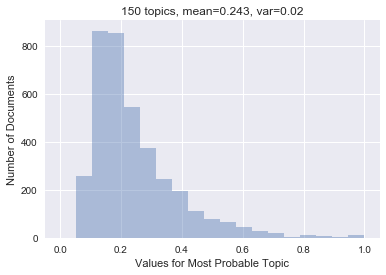
\includegraphics[width=7cm]{gfx/Hyperparams/150topics_English_nmf.png}
		\caption{Count of the value of the most probable topic, summed over all topics.}
		\label{fig:mean}
	\end{minipage}%
	\begin{minipage}[b]{0.5\textwidth}
		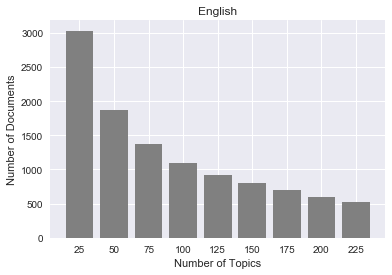
\includegraphics[width=7cm]{gfx/Hyperparams/English_nmf_Comments.png}
		\caption{Number of documents the topics are expressed above the threshold}
		\label{fig:topic number}
	\end{minipage}
\end{figure}	

After finding the appropriate topic number, the Topic Models generated with \ac{NMF} and \ac{LDA} for the same dataset were inspected manually. The domain experts labeled the topics and the Topic Model with the higher number of labels was chosen. The final selection of the Topic Models is shown in Table \ref{tab:finaltopics_editorial_forums}. And the Topic Models for the summarized comments is shown in Table \ref{tab:editoria_comments}. \\


%Editorial and Forums
\begin{table}[h]
	\centering
	\makebox[0pt][c]{\parbox{1.0\textwidth}{%
		\begin{minipage}[b]{0.5\textwidth}
			\begin{tabular}[b]{lcc}
				\cmidrule{2-3}  & Editorial articles & Comments
				\\ \midrule
				German    & \textbf{190} &    \textit{125}       \\
				English    & \textbf{130}  &      \textit{125}       \\ 
				\bottomrule
			\end{tabular}
		\end{minipage}
		\hfill

		\begin{minipage}[b]{0.5\textwidth}
			\begin{tabular}[b]{lccc}
				\cmidrule{2-4}  & \multicolumn{2}{c}{Editorials} & \multirow{2}{*}{Forums} \\
				\cmidrule(r){2-3}
				\cmidrule(r){2-3}
				& articles     &    comments       &                         
				\\ \midrule
				& \textbf{190} &  \textit{170}    &      \textit{170}       \\
				& \textbf{130} &  \textit{170}    &      \textbf{110}       \\ 
				\bottomrule
			\end{tabular}
		\end{minipage}
\vspace{1pt}
\caption[Final number of topics for Editorials and Forums]{The optimal number of topics for Editorials and Forums. \\
	\textit{Italic} denotes \ac{NMF} and \textbf{bold} numbers denote \ac{LDA}.}
\label{tab:finaltopics_editorial_forums}
}}
\end{table}
\newpage